\section*{BACKGROUND}

Power-system evaluation targets are shifting from stand-alone numerical algorithms toward tool-using systems that retrieve structured state, call analysis tools, and support human decision making. Large language models (LLMs) and agentic workflows are therefore increasingly explored for simulation orchestration, engineering question answering, and human-in-the-loop analytical support \cite{liu2023agentbench,jia2024enhancing}. At the same time, canonical power-system test cases remain indispensable for validating steady-state analysis methods, and software ecosystems such as MATPOWER and pandapower have made these benchmark networks broadly reusable across research and education \cite{zimmerman2011matpower,thurner2018pandapower}.

In the electric-power domain, recent efforts such as ElecBench illustrate the value of domain-specific benchmarks for LLM evaluation, but they emphasize broader dispatch-oriented or text-oriented tasks rather than engineering-complete power-flow scenario records whose numerical state can be queried and graded programmatically \cite{zhou2024elecbench}. For power-system agent development, this leaves a practical gap between raw benchmark networks and benchmark-ready datasets.

The released \textit{pfbench v\datasetversion} dataset addresses this gap by packaging reproducibly perturbed power-flow scenarios into archival scenario records and benchmark-facing question items. The current frozen release contains \datasetscenarios{} solved scenarios and \datasetquestions{} question items across \datasetcases{} benchmark cases and \datasetfamilies{} structured query families, with an explicit failed-scenario log retained for transparency even when no scenario fails in the frozen package. Each scenario record stores the grid reference, a base-grid snapshot, the exact mutation specification, the full post-mutation input state, AC and DC solver outputs, provenance fields, and validation metadata. Each question item references its parent scenario and adds a prompt, a response schema, a solver-derived gold answer, and a programmatic grading policy. The design deliberately separates engineering truth from benchmark presentation: the solver produces truth, the scenario record preserves state, the question item exposes the evaluation interface, and the grader computes the score.

A second requirement is methodological credibility. For numerical power-flow benchmarks, reproducibility is not only a matter of seeded generation and deterministic grading; it also benefits from an external check against an independent software stack. Accordingly, the frozen release couples in-repository truth generation with a separate pandapower-based cross-validation stage. The canonical archived answers remain those produced by the release-generation solvers, while pandapower provides an external numerical consistency check over the same mutated scenarios.

This release is best understood as a dataset and benchmark descriptor rather than a software-method paper. Its primary contribution is the frozen dataset collection together with the supporting schemas, validation artifacts, cross-validation reports, checksums, and release metadata. The dataset is designed for tool-assisted or structured-context evaluation rather than unconstrained closed-book question answering. This framing is important for power-system agents because the relevant evaluation object is often not a natural-language prompt alone, but a pair consisting of \emph{(i)} a solved engineering scenario and \emph{(ii)} a structured task defined over that scenario. The release also follows a FAIR-oriented packaging posture by including machine-readable schemas, explicit field dictionaries, archival exports in JSONL and Parquet, release notes, and checksum-based integrity files \cite{wilkinson2016fair}.

The remainder of the paper describes the collection workflow, the external and internal validation design, the released record model, and the intended scope of reuse.

\section*{COLLECTION METHODS AND DESIGN}

\subsubsection*{Overview}

Fig.~\ref{fig:pipeline} summarizes the release-generation workflow. Starting from standard transmission test cases, the generator samples seeded mutations, solves the mutated network with AC and DC power flow, writes an engineering-complete scenario record, derives benchmark questions from solver truth, and freezes the package together with schemas, validation artifacts, and release metadata. In the finalized workflow, the freeze stage also runs an external pandapower-based cross-validation pass over the same mutated scenarios. The result is a benchmark dataset that supports power-flow retrieval, comparison, and structured reasoning tasks under explicit scenario context.

\begin{figure}[!t]
\centering
\begin{tikzpicture}[node distance=7mm and 4mm, every node/.style={font=\footnotesize}]
  \tikzstyle{box}=[draw, rounded corners, align=center, minimum height=7mm, inner sep=2mm]
  \node[box, fill=blue!6] (case) {Base transmission\\test case};
  \node[box, fill=blue!6, below=of case] (mut) {Seeded mutation\\specification};
  \node[box, fill=blue!6, below=of mut] (solve) {AC/DC power-flow\\solution};
  \node[box, fill=green!8, right=16mm of solve] (record) {Scenario record\\(canonical artifact)};
  \node[box, fill=green!8, above=of record] (question) {Question items\\(benchmark interface)};
  \node[box, fill=orange!10, below=of record] (freeze) {Schemas, validation,\\cross-validation, metadata};

  \draw[-latex, thick] (case) -- (mut);
  \draw[-latex, thick] (mut) -- node[right, xshift=1mm]{load scaling, outage, tap change} (solve);
  \draw[-latex, thick] (solve) -- (record);
  \draw[-latex, thick] (record) -- (question);
  \draw[-latex, thick] (record) -- (freeze);
  \draw[-latex, thick] (question) -- (freeze);
\end{tikzpicture}
\caption{Overview of the \textit{pfbench} generation and release pipeline. The design enforces a strict separation between solver-derived truth, engineering-complete scenario records, benchmark-facing question items, and both internal and external validation metadata.}
\label{fig:pipeline}
\end{figure}

\subsection*{Source cases and release scope}

The frozen release is derived from standard benchmark transmission cases. The current package contains cases \texttt{case14}, \texttt{case30}, \texttt{case39}, \texttt{case57}, \texttt{case118}, \texttt{case145}, and \texttt{case300}. The smaller cases are stored as repository-native MATPOWER-style benchmark data structures, while the larger cases are obtained through pandapower-backed conversions of standard benchmark networks \cite{zimmerman2011matpower,thurner2018pandapower}. This design preserves the familiarity of established power-system test cases while packaging them in a benchmark-oriented data model suitable for downstream AI evaluation. It also means that pandapower appears in the pipeline in two distinct roles: as a conversion aid for some larger source networks and as an independent external validator for the frozen scenario solves.

\subsection*{Deterministic scenario generation}

Each scenario is created by deterministic seeded perturbation of a base case. Seeded generation governs mutation sampling, split assignment, bus and branch target selection, and scenario identifiers. The current release uses three mutation classes.

\textbf{1) \texttt{scale\_bus\_load}.} For selected buses with nonzero load, active and reactive load are each multiplied by independently sampled factors in the interval $[0.9, 1.15]$. Each scenario contains two or three such load modifications, bounded by the number of buses with load.

\textbf{2) \texttt{line\_outage}.} With probability 0.45, one active branch is disabled, subject to a connectivity-preserving constraint. Candidate outages that disconnect the network are rejected and resampled.

\textbf{3) \texttt{set\_tap\_ratio}.} With probability 0.50, one branch with a nontrivial tap ratio is modified by scaling its tap ratio by a factor in $[0.96, 1.04]$.

Across the released scenarios, these rules produce 2641 load-scaling operations, 493 line outages, and 427 tap-ratio modifications. Human-readable summaries of the applied changes are stored in the scenario metadata to support prompt construction and auditability. A retry policy allows up to eight attempts per scenario seed if a sampled scenario cannot be solved successfully. No retry-exhausted scenarios remain in the released package.

\subsection*{Power-flow solution and truth generation}

The canonical scenario record is produced by in-repository solvers. The AC solution path uses an in-repository Newton--Raphson solver in polar coordinates (recorded solver name \texttt{newton\_raphson\_polar}) with tolerance $10^{-8}$ and a maximum of 30 iterations. The DC solution path uses an in-repository linear DC solver (recorded solver name \texttt{dc\_power\_flow}). Both solutions are stored for every released scenario, and gold answers are derived directly from these solver outputs rather than from an LLM or a post-hoc manual annotation process. This choice is central to the benchmark design because it makes the evaluation programmatic, deterministic, and reproducible.

\subsection*{External pandapower cross-validation}

To strengthen confidence in the released numerical results, the finalized workflow performs an external cross-validation pass with pandapower after scenario generation. Each mutated MATPOWER-style case is converted through \texttt{from\_ppc(...)}, solved with \texttt{runpp} for AC and \texttt{rundcpp} for DC, and then compared against the stored solver outputs. The cross-validation is intentionally external to the truth-generation path: the dataset's canonical answers remain the archived in-repository solver records, whereas pandapower acts as an independent numerical validator.

The validation layer includes several safeguards so that the comparison is like-for-like rather than superficially row-matched. First, if an inherited source case contains missing nominal-voltage metadata, the corresponding \texttt{base\_kV} values are filled only inside the pandapower conversion path so that the external solver can construct a valid network; the affected buses are recorded as preprocessing metadata rather than silently rewritten in the released scenario. Second, the mutated branch in-service state is explicitly reprojected onto the converted pandapower elements after \texttt{from\_ppc(...)} so that outaged lines and transformers preserve the intended topology. Third, bus and branch comparisons are aligned by original scenario identity rather than by internal row order, with pandapower line-, transformer-, and impedance-backed results mapped back to the original branch index. The resulting summary, per-scenario metrics, and Markdown report are defined as first-class release artifacts.

\subsection*{Question derivation}

Each solved scenario yields one question per query family, producing ten benchmark items per scenario. The released query families cover four direct retrieval tasks (bus voltage magnitude, bus voltage angle, branch active flow, branch reactive flow), four extremum tasks (minimum bus voltage magnitude, maximum absolute bus voltage angle, maximum absolute branch active flow, maximum absolute branch reactive flow), one AC--DC comparison task, and one condition-detection task for voltage-limit violations after excluding inherited source-case voltage-limit inconsistencies. These tasks were chosen to cover both simple table lookup and modest aggregation or comparison over the solved network state, without requiring free-form judgment or an LLM-based evaluator.

\section*{VALIDATION AND QUALITY}

The release is validated at four levels. First, the package is structurally validated against frozen schemas: all \datasetscenarios{} scenario records validate against the scenario schema, all \datasetquestions{} question items validate against the question schema, and all \datasetquestions{} \texttt{gold\_answer} objects validate against their item-specific \texttt{response\_schema}. Second, identity and leakage checks confirm that scenario identifiers are unique, question identifiers are unique, every question references a known scenario, all questions derived from the same scenario remain in the same split, and no cross-split scenario leakage is present. Third, completeness checks verify that every released scenario contains a base-grid snapshot, a post-mutation input state, a bus partition, AC results, DC results, and mutated bus, generator, and branch snapshots.

Fourth, the frozen scenarios are numerically cross-validated against pandapower. For each released scenario, the mutated MATPOWER-style case is converted to a pandapower network, solved with \texttt{runpp} for AC and \texttt{rundcpp} for DC, and compared against the stored solver results. The comparison covers AC bus voltage magnitude and angle, bus-level active and reactive generation totals, from-side and to-side AC branch flows, DC bus voltage angles, bus-level DC active generation totals, and DC branch active flows. The validation configuration uses explicit tolerances, namely $10^{-4}$ p.u. for AC voltage magnitudes, $10^{-2}$ degrees for bus voltage angles, $10^{-4}$ MW for bus-level generation totals, $10^{-3}$ MW for active branch flows, and $10^{-2}$ MVAr for reactive branch flows. To ensure like-for-like comparison, the validation layer (i) fills missing nominal-voltage metadata only inside the pandapower conversion path when required, (ii) explicitly reapplies mutated branch in-service flags after \texttt{from\_ppc(...)} so that outaged branches and transformers preserve the intended topology, and (iii) aligns bus and branch comparisons by original scenario identity rather than internal row order. Release packaging is configured to fail if any scenario exceeds the declared tolerances.

Table~\ref{tab:validation} summarizes the principal validation checks. In addition to schema-level validation and external numerical cross-validation, the package includes SHA-256 digests for integrity verification. The accompanying test suite passed 16 tests covering imports, case loading, generation-pipeline behavior, schema validation, CLI behavior, release-package creation, and pandapower-backed cross-validation regression cases.

The package also records numerical coverage across its solved scenarios. Total load spans from 186.19 MW to 291{,}192.16 MW, total scheduled generation spans from 189.21 MW to 343{,}735.10 MW, and absolute from-side branch active and reactive flows reach 9841.73 MW and 3004.01 MVAr, respectively. In addition, scenario records expose explicit \texttt{data\_quality\_flags} for inherited source-case artifacts, including missing nominal-voltage metadata, source voltage-limit inconsistencies, source generator reactive-limit inconsistencies, missing branch ratings, and AC/DC power-balance residuals. These ranges and quality annotations demonstrate that the released package covers both small teaching cases and substantially larger solved systems under nontrivial perturbations while preserving source-case fidelity.

Finally, the release design avoids a common source of benchmark ambiguity: no LLM is used as the source of truth and no LLM judge is required for grading. Scoring is computed by explicit programmatic graders, including numeric-tolerance checks, exact JSON checks, and argmin/argmax or ranking rules. This strengthens the methodological position of the dataset for reproducible benchmarking.

\begin{table}[!t]
\caption{Release validation summary for \textit{pfbench v\datasetversion}.}
\label{tab:validation}
\centering
\resizebox{\columnwidth}{!}{%
\begin{tabular}{p{0.33\columnwidth}p{0.20\columnwidth}p{0.36\columnwidth}}
\toprule
Validation check & Result & Evidence in release package \\
\midrule
Scenario schema validation & 1060/1060 pass & \texttt{VALIDATION\_SUMMARY.json} \\
Question schema validation & 10600/10600 pass & \texttt{VALIDATION\_SUMMARY.json} \\
Gold-answer schema validation & 10600/10600 pass & \texttt{VALIDATION\_SUMMARY.json} \\
Scenario IDs unique & Pass & \texttt{VALIDATION\_SUMMARY.json} \\
Question IDs unique & Pass & \texttt{VALIDATION\_SUMMARY.json} \\
Cross-split scenario leakage & None detected & \texttt{VALIDATION\_SUMMARY.json} \\
Completeness of scenario records & 1060/1060 complete & \texttt{QUALITY\_REPORT.md} \\
External pandapower cross-validation & Required; release build fails on tolerance violation & \texttt{CROSS\_VALIDATION\_SUMMARY.json}, \texttt{cross\_validation\_results.jsonl}, \texttt{CROSS\_VALIDATION\_REPORT.md} \\
Checksum verification & Pass & \texttt{CHECKSUMS.sha256} \\
Local test suite & 16 tests passed & repository test logs \\
\bottomrule
\end{tabular}}
\end{table}

\section*{RECORDS AND STORAGE}


The release package occupies approximately 250 MB on disk and is organized as a frozen directory intended for archival deposition. Core benchmark data are distributed as JSONL and Parquet files for scenario records, question items, and failed-scenario logs. Supporting metadata include a machine-readable manifest, an internal validation summary, pandapower cross-validation summaries and reports, FAIR-style metadata, checksums, release notes, a field dictionary, schema documentation, reference records, configuration files, and the frozen JSON schemas for both main artifact types.

Fig.~\ref{fig:record-model} illustrates the data model. The scenario record is the canonical engineering artifact. It stores base-case identity, the pre-mutation grid snapshot, the mutation specification, the post-mutation system state, explicit data-quality flags, AC and DC solver outputs, provenance fields, and metadata. The question item is the benchmark-facing artifact. It references the parent scenario through \texttt{scenario\_id} and adds the prompt, response schema, gold answer, grader, and benchmark metadata. This one-to-many structure avoids duplicating the full grid state in every question item while retaining an explicit link to the underlying solved scenario.

\begin{figure}[!t]
\centering
\begin{tikzpicture}[node distance=6mm and 4mm, every node/.style={font=\footnotesize}]
  \tikzstyle{box}=[draw, rounded corners, minimum height=6.5mm, inner sep=2mm, align=left]
  \node[box, fill=green!8, text width=0.42\columnwidth] (scenario) {\textbf{Scenario record}\\
  \texttt{scenario\_id}\\
  \texttt{grid\_reference}\\
  \texttt{base\_grid\_snapshot}\\
  \texttt{scenario\_spec}\\
  \texttt{scenario\_input\_state}\\
  \texttt{data\_quality\_flags}\\
  \texttt{powerflow\_results}\\
  \texttt{provenance}, \texttt{metadata}};

  \node[box, fill=blue!7, right=6mm of scenario, text width=0.34\columnwidth] (question1) {\textbf{Question item A}\\
  \texttt{question\_id}\\
  \texttt{scenario\_id}\\
  \texttt{query\_family}\\
  \texttt{prompt}\\
  \texttt{gold\_answer}\\
  \texttt{grader}};

  \node[box, fill=blue!7, below=of question1, text width=0.34\columnwidth] (question2) {\textbf{Question item B}\\
  Same parent scenario,\\different task family};

  \node[box, fill=blue!7, below=of question2, text width=0.34\columnwidth] (question3) {\textbf{Question item C}\\
  Same parent scenario,\\different response schema};

  \draw[-latex, thick] (scenario.east) -- (question1.west);
  \draw[-latex, thick] (scenario.east) -- (question2.west);
  \draw[-latex, thick] (scenario.east) -- (question3.west);
\end{tikzpicture}
\caption{Relationship between the two principal artifact types. One scenario record preserves complete engineering state, while multiple question items reference the same \texttt{scenario\_id} to expose benchmark tasks without duplicating the full network description.}
\label{fig:record-model}
\end{figure}

Table~\ref{tab:overview} summarizes the release. Table~\ref{tab:casecoverage} lists the case coverage and per-case counts. Table~\ref{tab:taxonomy} enumerates the query families, task types, result-table dependencies, and grading modes.

\begin{table}[!t]
\caption{Overview of the frozen \textit{pfbench v\datasetversion} release.}
\label{tab:overview}
\centering
\begin{tabular}{p{0.44\columnwidth}p{0.46\columnwidth}}
\toprule
Item & Value \\
\midrule
Dataset identifier & \texttt{pfbench} \\
Dataset version & \datasetversion{} \\
Question schema version & 0.3.0 \\
Scenario schema version & 0.5.0 \\
Solved scenarios & \datasetscenarios{} \\
Question items & \datasetquestions{} \\
Benchmark cases & \datasetcases{} \\
Query families & \datasetfamilies{} \\
Failed scenarios in release & \datasetfails{} \\
Questions per scenario & 10 \\
Primary formats & JSONL, Parquet, JSON Schema, Markdown, YAML \\
Approximate package size & 250 MB \\
\bottomrule
\end{tabular}
\end{table}

\begin{table}[!t]
\caption{Case coverage in the frozen release.}
\label{tab:casecoverage}
\centering
\resizebox{\columnwidth}{!}{%
\begin{tabular}{lccc}
\toprule
Case & Nominal buses & Solved scenarios & Question items \\
\midrule
\texttt{case14} & 14 & 220 & 2200 \\
\texttt{case30} & 30 & 220 & 2200 \\
\texttt{case39} & 39 & 190 & 1900 \\
\texttt{case57} & 57 & 190 & 1900 \\
\texttt{case118} & 118 & 150 & 1500 \\
\texttt{case145} & 145 & 60 & 600 \\
\texttt{case300} & 300 & 30 & 300 \\
\bottomrule
\end{tabular}}
\end{table}

\begin{table}[!t]
\caption{Query-family taxonomy and grading modes.}
\label{tab:taxonomy}
\centering
\resizebox{\columnwidth}{!}{%
\begin{tabular}{p{0.31\columnwidth}p{0.16\columnwidth}p{0.18\columnwidth}p{0.19\columnwidth}}
\toprule
Query family & Task type & Required result table & Grading mode \\
\midrule
\texttt{direct\_bus\_vm} & retrieval & AC bus & numeric tolerance \\
\texttt{direct\_bus\_va} & retrieval & AC bus & numeric tolerance \\
\texttt{argmin\_bus\_vm} & extremum & AC bus & argmin \\
\texttt{argmax\_bus\_va\_abs} & extremum & AC bus & argmax \\
\texttt{direct\_branch\_p\_from} & retrieval & AC branch & numeric tolerance \\
\texttt{direct\_branch\_q\_from} & retrieval & AC branch & numeric tolerance \\
\texttt{max\_branch\_abs\_p\_from} & extremum & AC branch & argmax \\
\texttt{max\_branch\_abs\_q\_from} & extremum & AC branch & argmax \\
\texttt{compare\_ac\_dc\_branch\_p\_from} & comparison & AC+DC branch & exact JSON / tolerance \\
\texttt{is\_voltage\_violation\_present} & condition detection & AC bus + limits & exact JSON \\
\bottomrule
\end{tabular}}
\end{table}

Listing~\ref{lst:scenario} shows an abbreviated scenario record. The full release documentation includes a field dictionary and JSON schemas that define the exact field types and required keys.

\begin{lstlisting}[caption={Abbreviated scenario record showing the major top-level keys in the canonical engineering artifact.},label={lst:scenario}]
{
  "dataset_id": "pfbench",
  "scenario_id": "...",
  "source_case": "case57",
  "split": "dev",
  "grid_reference": {...},
  "base_grid_snapshot": {...},
  "scenario_spec": {
    "seed": 170050,
    "mutations": [
      {"op": "scale_bus_load", ...},
      {"op": "line_outage", ...}
    ]
  },
  "scenario_input_state": {...},
  "data_quality_flags": {...},
  "powerflow_results": {
    "ac": {...},
    "dc": {...}
  },
  "provenance": {...},
  "metadata": {...}
}
\end{lstlisting}

\begin{figure}[!t]
\centering
\subfloat[Scenarios per case.]{%
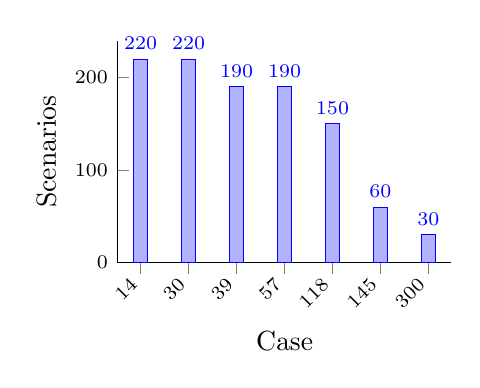
\begin{tikzpicture}
\begin{axis}[
    width=0.48\columnwidth,
    height=4.4cm,
    ybar,
    bar width=5pt,
    ymin=0,
    ymax=240,
    xtick=data,
    xticklabels={14,30,39,57,118,145,300},
    xticklabel style={font=\scriptsize, rotate=45, anchor=east},
    yticklabel style={font=\scriptsize},
    xlabel={Case}, ylabel={Scenarios},
    nodes near coords,
    every node near coord/.append style={font=\scriptsize},
    axis lines*=left,
    enlarge x limits=0.08
]
\addplot coordinates {(0,220) (1,220) (2,190) (3,190) (4,150) (5,60) (6,30)};
\end{axis}
\end{tikzpicture}}
\hfill
\subfloat[Question split composition.]{%
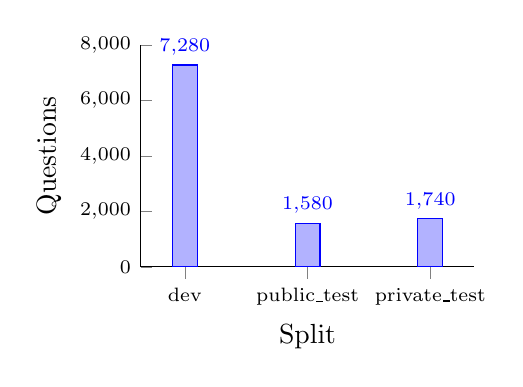
\begin{tikzpicture}
\begin{axis}[
    width=0.48\columnwidth,
    height=4.4cm,
    ybar,
    bar width=9pt,
    ymin=0,
    ymax=8000,
    symbolic x coords={dev,public_test,private_test},
    xticklabels={dev,public\_test,private\_test},
    xtick=data,
    xticklabel style={font=\scriptsize},
    yticklabel style={font=\scriptsize},
    xlabel={Split}, ylabel={Questions},
    nodes near coords,
    every node near coord/.append style={font=\scriptsize},
    axis lines*=left,
    enlarge x limits=0.18
]
\addplot coordinates {(dev,7280) (public_test,1580) (private_test,1740)};
\end{axis}
\end{tikzpicture}}
\caption{Coverage statistics of the frozen release. All ten questions derived from a given scenario are assigned to the same split, preventing cross-split scenario leakage.}
\label{fig:coverage}
\end{figure}

\section*{REUSE, SCOPE, AND LIMITATIONS}

The current release is best understood as a structured benchmark for reasoning over solved power-flow scenarios. It is \emph{not} intended as free-form closed-book question answering over textual descriptions alone. Instead, the evaluation mode stored in the release is \texttt{tool\_or\_structured\_context\_required}, meaning that a system under test is expected to access the provided scenario record or an equivalent structured solver context. This assumption aligns well with emerging power-system agents, which are valuable not because they memorize numerical answers, but because they can retrieve, summarize, compare, and reason over structured engineering state.

An important consequence of the revised validation design is that the benchmark no longer depends on a single numerical pathway. The released scenario record preserves the canonical answer key, while the pandapower cross-validation artifacts provide an external check on topology handling and numerical consistency. For agent evaluation, this improves trustworthiness: a model is not asked to match opaque annotations, but to reason over records whose provenance and validation trail are explicit.

Several reuse paths follow directly from this design. First, the dataset can be used for structured-output evaluation, where a model must return JSON that satisfies a response schema and matches a solver-derived answer. Second, the scenario records can serve as tool-ready contexts for agent development, including agents that retrieve a scenario, inspect relevant result tables, and answer questions without rerunning the solver. Third, the deterministic split policy and explicit provenance enable controlled ablation studies over case size, mutation type, query family, and split. Fourth, the package is suitable for archival deposition because it includes versioning, checksums, machine-readable schemas, cross-validation artifacts, and documentation aligned with FAIR-style reuse practices \cite{wilkinson2016fair}.

The release also has clear boundaries. The package is derived from standard benchmark cases rather than operational utility data. The AC and DC solvers are in-repository implementations intended for reproducible dataset generation, not complete production-grade analysis suites. The AC solve path assumes exactly one slack bus and does not enforce generator reactive-power limits. The current mutation family is limited to load scaling, connectivity-preserving line outages, and tap-ratio adjustments; it does not yet include generator outages, redispatch, or broader operating actions. These limitations do not negate the dataset's usefulness, but they define its present scope.

Relative to neighboring efforts, \textit{pfbench} is complementary rather than competitive. AgentBench provides a general framework for benchmarking LLM agents across interactive environments \cite{liu2023agentbench}. ElecBench demonstrates the value of domain-specific power benchmarks for LLM evaluation \cite{zhou2024elecbench}. \textit{pfbench} contributes a narrower but deeper artifact: solver-grounded, engineering-complete power-flow scenarios with frozen benchmark questions, programmatic grading, and explicit external numerical cross-validation. This design is well matched to power-system agent development, where numerical state fidelity, provenance, and reproducibility matter as much as linguistic fluency.

\section*{CODE AVAILABILITY AND REPRODUCIBILITY}

The dataset is accompanied by a public source repository for scenario generation, internal validation, external pandapower cross-validation, and release packaging. The repository contains the case loaders, mutation engine, AC and DC solvers, question-generation logic, schema definitions, validation utilities, test suite, and command-line interface used to build the release. For long-term reuse, both the dataset package and the companion source repository should be deposited in persistent external repositories and cited through DOI-backed records. In the manuscript files provided here, the dataset DOI and code-repository DOI are left as explicit placeholders because external deposition is still pending.

The release can be regenerated and verified through a short command sequence, shown in Listing~\ref{lst:commands}. These commands create the environment, run the test suite, build the frozen release package, execute the standalone pandapower cross-validation command, generate a summary report, and verify the checksums. The standalone \texttt{cross-validate} command remains useful even though release builds already generate the archived cross-validation artifacts, because it allows the external check to be rerun or inspected independently. The release package also includes \texttt{README.md}, \texttt{FIELD\_DICTIONARY.md}, and \texttt{SCHEMA\_DOCS.md} so that downstream users can understand the file inventory, environment requirements, and expected outputs before using the dataset.

\begin{lstlisting}[language=bash,caption={Representative commands for reproducing, cross-validating, and packaging the frozen release. Repository and DOI placeholders should be replaced before submission.},label={lst:commands}]
conda env create -f environment.yml
conda activate pfbench
pytest -q
pfbench build-release --config configs/release_v1.yaml \
  --out datasets/pfbench/v1
pfbench cross-validate --scenarios datasets/pfbench/v1/scenarios.jsonl
pfbench report --dataset datasets/pfbench/v1/questions.jsonl
cd datasets/pfbench/v1
sha256sum -c CHECKSUMS.sha256
\end{lstlisting}

The companion code repository should be cited in the final version using a persistent identifier, for example through Zenodo or a comparable archive. Until that deposition is complete, the manuscript should retain explicit placeholders such as \url{https://doi.org/TBD} for the dataset and \url{https://github.com/TBD/pfbench} for the source repository, then replace them immediately prior to submission.

\balance
\section*{ACKNOWLEDGEMENTS AND INTERESTS}


\textbf{Funding:} This work is supported by the startup fund of the Department of Electrical and Computer Engineering, Kansas State University.

\textbf{External data and software attribution:} The release is derived from standard benchmark cases and conversions associated with MATPOWER and pandapower \cite{zimmerman2011matpower,thurner2018pandapower}. 
The present package distributes derived benchmark artifacts and release metadata rather than full upstream source distributions.
